% Compilar desde el directorio docs/:
%   cd docs && pdflatex partial.tex && pdflatex partial.tex
% (dos pasadas para que se resuelvan las referencias cruzadas)

\documentclass[11pt,a4paper]{article}

\usepackage[utf8]{inputenc}
\usepackage[T1]{fontenc}
\usepackage[spanish,es-tabla,es-noshorthands]{babel}
\usepackage{lmodern}
\usepackage[margin=2.4cm]{geometry}
\usepackage{amsmath,amssymb}
\usepackage{graphicx}
\usepackage{booktabs}
\usepackage{array}
\usepackage{tabularx}
\usepackage{caption}
\usepackage{enumitem}
\usepackage{siunitx}
\sisetup{group-separator={\,},group-minimum-digits=4}
\usepackage{hyperref}
\usepackage{tikz}
\usetikzlibrary{positioning,shapes.geometric,fit,backgrounds}

\graphicspath{{figures/}}

\hypersetup{
  colorlinks=true,
  linkcolor=black,
  urlcolor=blue!60!black,
  citecolor=black
}

\setlength{\parskip}{0.5em}
\setlength{\parindent}{0pt}

\begin{document}

% =====================================================================
\begin{titlepage}
  \centering
  \vspace*{1.5cm}

  
\includegraphics[width=0.55\linewidth]{uniandes-logo.png}\\[2.0cm]

  {\large Facultad de Ingeniería\par}
  \vspace{0.2cm}
  {\normalsize Maestría en Inteligencia Artificial (MAIA)\par}
  \vspace{0.2cm}
  {\normalsize Aprendizaje por Refuerzo\par}

  \vspace{2.5cm}

  \rule{0.85\linewidth}{0.5pt}\\[0.7cm]
  {\LARGE \textbf{Entrega parcial}\par}
  \vspace{0.3cm}
  {\Large Ambiente, estados y acciones\par}
  \vspace{0.7cm}
  \rule{0.85\linewidth}{0.5pt}

  \vfill

  {\large Juan David Lara Camacho\par}
  \vspace{0.2cm}
  {\large Agustín Serrano\par}

  \vspace{1.5cm}

  {\normalsize Universidad de los Andes\par}
  {\normalsize \today\par}

  \vspace{0.5cm}
\end{titlepage}

% =====================================================================
\begin{abstract}
\noindent
Modelamos el ambiente \texttt{MiniGrid-BlockedUnlockPickup-v0} como un proceso
de decisión de Markov determinista para entrenar un agente Q-learning tabular.
La tarea exige una secuencia obligatoria de subtareas: mover una bola que
bloquea la puerta, recoger la llave, abrir la puerta, soltar la llave y, por
último, recoger la caja objetivo. La representación del estado tiene que
capturar tanto la posición y orientación del agente como el progreso ya
alcanzado en el episodio. Definimos el estado con ocho componentes, las seis
acciones discretas que ofrece MiniGrid y una función de recompensa con
\emph{shaping} por subtareas que suma a lo más \(+2.80\) por episodio. Con
esta formulación el agente alcanza \(100/100\) de éxito en evaluación greedy
en 24 pasos.
\end{abstract}

% =====================================================================
\section{Introducción}
\label{sec:intro}

El proyecto del curso pide modelar y resolver un problema con aprendizaje por
refuerzo siguiendo el marco estándar de los procesos de decisión de Markov
\cite{sutton}. Esta entrega cubre la primera parte: la definición formal del
ambiente. La rúbrica pide tres cosas:
\begin{enumerate}[leftmargin=*]
  \item el conjunto de estados \(\mathcal{S}\) que captura toda la información
        relevante para decidir,
  \item el conjunto de acciones \(\mathcal{A}\) y el comportamiento esperado
        del agente,
  \item el modelo de recompensa expresado como tripletas
        \((s, a, s')\mapsto r\).
\end{enumerate}

Para esta entrega elegimos modelar el ambiente
\texttt{MiniGrid-BlockedUnlockPickup-v0} de la librería MiniGrid
\cite{minigrid}. Su estructura de subtareas (mover una bola que bloquea una
puerta, recoger una llave, abrir la puerta, soltar la llave y recoger una
caja objetivo) obliga a un diseño de estado y de recompensa con varias
variables auxiliares, dependencias de orden entre subtareas y
\emph{shaping} de la señal de aprendizaje. El resto del documento desarrolla
formalmente la definición del ambiente sobre el que entrenamos el agente.

% =====================================================================
\section{Ambiente: \texttt{MiniGrid-BlockedUnlockPickup-v0}}
\label{sec:ambiente}

El ambiente es una grilla rectangular con dos cuartos separados por un muro
vertical y conectados por una sola casilla con puerta. El agente parte en el
cuarto izquierdo y debe llegar a una casilla objetivo en el cuarto derecho.
La puerta está cerrada y necesita una llave del mismo color. Además, hay
una bola del mismo color que la puerta justo enfrente, bloqueando el
acceso. La Figura~\ref{fig:env_schematic} muestra el esquema general del
ambiente y la Figura~\ref{fig:env_frames} cinco fotogramas de un episodio
greedy ya resuelto.

Dos detalles del ambiente subyacente (la implementación
\texttt{MiniGrid-BlockedUnlockPickup-v0}) conviene fijarlos desde ahora,
porque condicionan el conjunto de acciones y la condición de terminación
que aparecen más adelante. Primero, retirar la bola que bloquea la puerta
se hace recogiéndola con \texttt{pickup} y soltándola en otra celda con
\texttt{drop}: en MiniGrid no existe una acción de empujar, así que la
única forma de despejar la bola es usar el inventario (que admite un solo
objeto a la vez). Segundo, la casilla objetivo del cuarto derecho está
materializada en el ambiente como la celda donde se encuentra la caja
(\texttt{box}). El ambiente dispara \texttt{terminated=True} cuando el
agente la recoge. Por eso nuestro modelo incluye \texttt{drop} entre las
acciones y usa \texttt{box\_picked} como condición terminal.

\begin{figure}[h]
  \centering
  \begin{tikzpicture}[every node/.style={font=\small}]
    % Fondos de los cuartos
    \fill[blue!4]   (0,0) rectangle (6,5);
    \fill[orange!4] (6,0) rectangle (12,5);

    % Muros externos e interno con hueco para la puerta
    \draw[thick] (0,0) rectangle (12,5);
    \draw[thick] (6,0) -- (6,2);
    \draw[thick] (6,3) -- (6,5);

    % Puerta y etiqueta
    \draw[green!55!black, line width=2.5pt] (6,2.05) -- (6,2.95);
    \node[green!55!black, font=\small\itshape, anchor=west]
      at (6.15, 2.5) {puerta};

    % Títulos de cuartos
    \node[font=\small\bfseries] at (3,   5.45) {Cuarto izquierdo};
    \node[font=\small\bfseries] at (9,   5.45) {Cuarto derecho};

    % Llave (verde, esquina superior izquierda)
    \fill[green!55!black] (1.2, 3.8) circle (0.22);
    \node[font=\footnotesize, anchor=north] at (1.2, 3.45) {llave};

    % Agente (triángulo rojo orientado a la derecha)
    \draw[fill=red!75, draw=red!85!black]
      (1.6, 1.4) -- (2.3, 1.85) -- (1.6, 2.3) -- cycle;
    \node[font=\footnotesize, anchor=north] at (1.95, 1.05) {agente};

    % Bola (azul, en frente de la puerta)
    \fill[blue!75] (4.6, 2.5) circle (0.25);
    \node[font=\footnotesize, anchor=north] at (4.6, 2.05) {bola};

    % Caja (morada, esquina superior derecha)
    \draw[purple!85, line width=2pt, fill=purple!8]
      (10.0, 3.5) rectangle (10.7, 4.2);
    \node[font=\footnotesize, anchor=north] at (10.35, 3.2) {caja};
  \end{tikzpicture}
  \caption{Esquema del ambiente. Dos cuartos separados por un muro vertical
  con una sola casilla de paso (la puerta). Las dimensiones exactas, los
  anchos de cuarto y las posiciones iniciales de los objetos se aleatorizan
  al reiniciar el ambiente; fijamos la semilla del generador para que cada
  ejecución arranque desde la misma configuración. El color de la puerta y
  de la llave también se aleatoriza por episodio: en nuestra semilla
  salieron verdes (los frames de la Figura~\ref{fig:env_frames} muestran
  esa misma ejecución).}
  \label{fig:env_schematic}
\end{figure}

\begin{figure}[h]
  \centering
  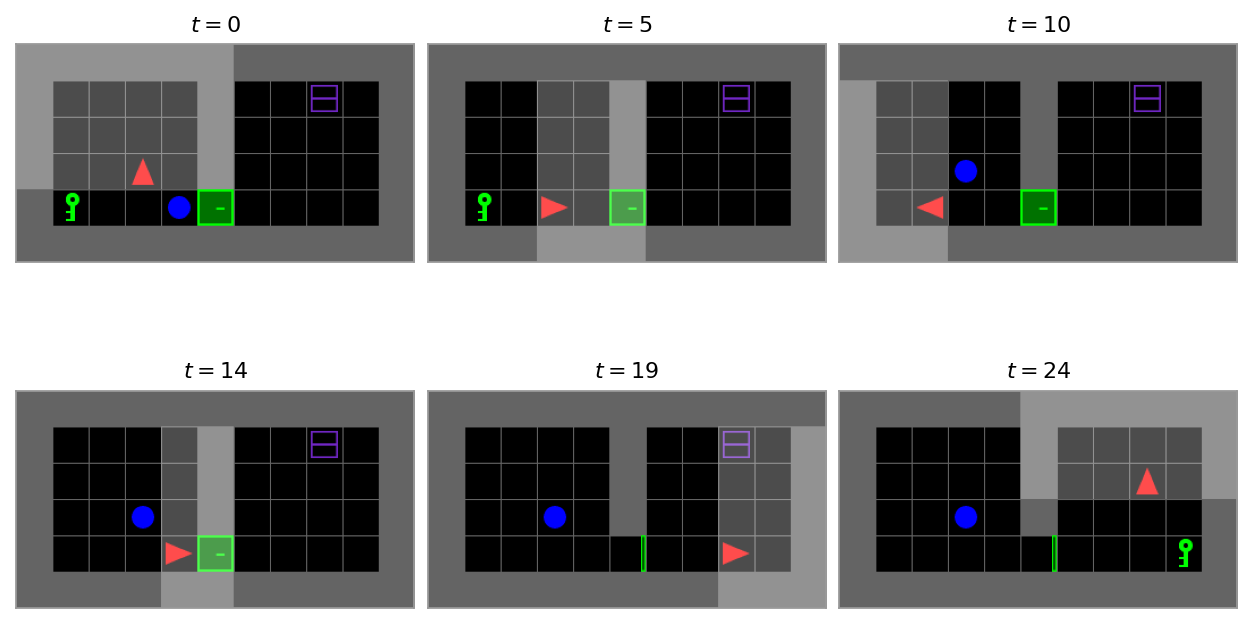
\includegraphics[width=\linewidth]{minigrid_greedy_frames.png}
  \caption{Seis fotogramas equiespaciados de un episodio greedy del agente
  entrenado, en orden de izquierda a derecha y de arriba a abajo. La fila
  superior cubre la fase en el cuarto izquierdo: en \(t=0\) el agente parte
  desde su posición inicial, en \(t=5\) la bola ya fue retirada de enfrente
  de la puerta y en \(t=10\) el agente carga la llave camino al umbral. La
  fila inferior cubre la fase en el cuarto derecho: en \(t=14\) la puerta
  está abierta y el agente la cruza, en \(t=19\) avanza hacia la caja y en
  \(t=24\) la recoge, lo que termina el episodio.}
  \label{fig:env_frames}
\end{figure}

La tarea no se puede resolver sin completar las subtareas en un orden fijo:
mover la bola, recoger la llave, abrir la puerta, recoger la caja. El
ambiente no admite atajos. La Figura~\ref{fig:subtasks} formaliza esa
secuencia.

\begin{figure}[h]
  \centering
  \begin{tikzpicture}[
    node distance=12mm and 9mm,
    every node/.style={font=\small},
    state/.style={draw, rounded corners=2pt, minimum height=9mm,
                  minimum width=22mm, inner sep=4pt, fill=gray!8},
    goalstate/.style={draw, rounded corners=2pt, minimum height=9mm,
                  minimum width=22mm, inner sep=4pt, fill=green!12}
  ]
    % Fila superior: inicio -> bola -> llave -> puerta
    \node[state] (s0) {inicio};
    \node[state, right=of s0] (s1) {bola movida};
    \node[state, right=of s1] (s2) {llave en mano};
    \node[state, right=of s2] (s3) {puerta abierta};

    % Fila inferior, alineada con la superior pero leída de derecha a izquierda
    \node[state, below=of s3] (s4) {llave soltada};
    \node[state, left=of s4]  (s5) {caja en mano};
    \node[goalstate, left=of s5] (s6) {goal};

    % Conexiones
    \draw (s0) -- (s1);
    \draw (s1) -- (s2);
    \draw (s2) -- (s3);
    \draw (s3) -- (s4);
    \draw (s4) -- (s5);
    \draw (s5) -- (s6);
  \end{tikzpicture}
  \caption{Cadena de subtareas que el agente debe completar. La fila
  superior se lee de izquierda a derecha y la fila inferior de derecha a
  izquierda, siguiendo el orden temporal de los eventos. Cada conexión
  representa el cambio que se produce la primera vez que una acción
  modifica ese aspecto del estado dentro del episodio.}
  \label{fig:subtasks}
\end{figure}

Algunos parámetros del ambiente que conviene fijar de entrada. El horizonte
máximo de un episodio es \texttt{max\_steps}\(=576\), valor por defecto del
ambiente. Las orientaciones se codifican como enteros \(0,1,2,3\) para Este,
Sur, Oeste y Norte. El ambiente es completamente determinista una vez fijada
la semilla del generador.

% =====================================================================
\section{Conjunto de estados}
\label{sec:estados}

\subsection{Definición formal}

Cada estado se representa como una tupla de ocho componentes:
\begin{equation}
  s = \big(\,
    \underbrace{(x,y)}_{\text{pos}},\;
    \underbrace{d}_{\text{dir}},\;
    \underbrace{c}_{\text{carrying}},\;
    \underbrace{b}_{\text{ball\_moved}},\;
    \underbrace{k_p}_{\text{key\_picked}},\;
    \underbrace{o}_{\text{door\_open}},\;
    \underbrace{k_d}_{\text{key\_dropped}},\;
    \underbrace{x_p}_{\text{box\_picked}}
  \,\big)
  \label{eq:state}
\end{equation}
La Tabla~\ref{tab:state} describe cada componente.

\begin{table}[h]
  \centering
  \small
  \setlength{\extrarowheight}{2pt}
  \begin{tabularx}{\linewidth}{l l l X}
    \toprule
    \textbf{Componente} & \textbf{Tipo} & \textbf{Rango} & \textbf{Descripción} \\
    \midrule
    \texttt{pos}          & \((\mathbb{Z}_{\ge 0})^2\) & \((0..W{-}1, 0..H{-}1)\) & posición del agente en la grilla \\
    \texttt{dir}          & \(\mathbb{Z}\) & \(\{0,1,2,3\}\) & orientación: 0 E, 1 S, 2 W, 3 N \\
    \texttt{carrying}     & cadena & \(\{\text{none, key, ball, box}\}\) & objeto que el agente lleva en el momento actual \\
    \texttt{ball\_moved}  & booleano & \(\{0,1\}\) & la bola ya no está en su posición inicial \\
    \texttt{key\_picked}  & booleano & \(\{0,1\}\) & el agente recogió la llave en algún momento del episodio \\
    \texttt{door\_open}   & booleano & \(\{0,1\}\) & la puerta está abierta \\
    \texttt{key\_dropped} & booleano & \(\{0,1\}\) & el agente soltó la llave después de abrir la puerta \\
    \texttt{box\_picked}  & booleano & \(\{0,1\}\) & el agente cargó la caja al menos una vez \\
    \bottomrule
  \end{tabularx}
  \caption{Componentes del estado. Las primeras cinco filas son lo que el
  agente puede observar directamente del ambiente. Las tres últimas son
  banderas de progreso que necesitamos para que la función de recompensa
  sea Markoviana sobre \((s, a, s')\); ver Sección~\ref{sec:recompensa}.}
  \label{tab:state}
\end{table}

\subsection{Justificación}

Las primeras cinco componentes son las obvias. La posición y la orientación
fijan qué celda mira el agente. El componente \texttt{carrying} indica qué
tiene en mano. Importa porque la acción \texttt{pickup} solo funciona con las
manos vacías. También importa qué objeto se está cargando, porque eso
restringe lo que se puede hacer a continuación. Las banderas
\texttt{ball\_moved} y \texttt{door\_open} son condiciones del ambiente que
el agente podría inducir mirando las celdas vecinas. Conviene exponerlas
explícitamente para que la Q-tabla las indexe sin ambigüedad.

Las tres últimas (\texttt{key\_picked}, \texttt{key\_dropped} y
\texttt{box\_picked}) parecen redundantes a primera vista:
\texttt{key\_picked} se podría deducir de \texttt{carrying = key} en el
momento del \texttt{pickup}, y \texttt{key\_dropped} de la combinación de
variables anteriores. Las incluimos por la \emph{recompensa}, no por la
representación del progreso físico. Nuestro \emph{shaping} entrega cada
bonificación una sola vez por episodio: la primera vez que se alcanza la
condición. Sin estas banderas, la misma transición \((s, a, s')\) podría
producir recompensas distintas según la historia previa del episodio. La
Sección~\ref{sec:recompensa} desarrolla este punto.

\subsection{Tamaño del espacio}

Una cota superior, tomando todos los productos cartesianos posibles, es
\(W \cdot H \cdot 4 \cdot 4 \cdot 2^5\). Para la configuración por defecto,
con grilla aproximadamente \(11\times 6\), eso da del orden de \(10^4\)
estados. La cota es laxa. Las restricciones de consistencia eliminan la
mayor parte de las combinaciones: \(\texttt{key\_dropped}=1\) implica
\(\texttt{door\_open}=1\) y \(\texttt{key\_picked}=1\), y
\(\texttt{box\_picked}=1\) implica las tres banderas anteriores. En
\num{10000} episodios de entrenamiento el agente visita \num{635} estados
distintos.

\subsection{Estado inicial y estados terminales}

El estado inicial \(s_0\) tiene posición y orientación fijas (las del
\texttt{reset()} con la semilla del experimento), \(\texttt{carrying} =
\text{none}\) y todas las banderas en cero. Un estado se vuelve terminal
cuando \(\texttt{box\_picked} = 1\): el ambiente devuelve
\texttt{terminated=True} y el agente recibe la recompensa terminal. Si en
cambio se alcanza \texttt{max\_steps} sin éxito, el ambiente devuelve
\texttt{truncated=True}; ese caso no se considera terminal en el sentido
del MDP, simplemente cierra el episodio por límite de tiempo.

% =====================================================================
\section{Conjunto de acciones}
\label{sec:acciones}

El conjunto de acciones es \(\mathcal{A} = \{0,1,2,3,4,5\}\) y corresponde a
las seis acciones discretas que MiniGrid expone para este tipo de tareas
\cite{minigrid}. Cada acción está definida en todo el espacio de estados,
pero solo produce un cambio efectivo de estado cuando se cumplen ciertas
condiciones locales. La Tabla~\ref{tab:actions} indica, para cada acción,
los estados en los que es aplicable y el efecto que produce.

\begin{table}[h]
  \centering
  \small
  \setlength{\extrarowheight}{3pt}
  \begin{tabularx}{\linewidth}{c l X X}
    \toprule
    \textbf{Idx} & \textbf{Nombre} & \textbf{Aplicable en} & \textbf{Efecto} \\
    \midrule
    0 & \texttt{left}    & todos los estados & \(d \mapsto (d-1) \bmod 4\) \\
    1 & \texttt{right}   & todos los estados & \(d \mapsto (d+1) \bmod 4\) \\
    2 & \texttt{forward} & estados con celda al frente transitable (vacía o puerta abierta) & avanza una celda en dirección \(d\) \\
    3 & \texttt{pickup}  & estados con \texttt{carrying = none} y un objeto recogible (llave, bola o caja) en la celda al frente & \texttt{carrying} toma el tipo del objeto, la celda queda vacía \\
    4 & \texttt{drop}    & estados con \texttt{carrying \(\neq\) none} y celda al frente vacía & deja el objeto en esa celda, \texttt{carrying} pasa a \texttt{none} \\
    5 & \texttt{toggle}  & estados con la puerta al frente y \texttt{carrying = key} & abre la puerta: \texttt{door\_open} pasa de \(0\) a \(1\) \\
    \bottomrule
  \end{tabularx}
  \caption{Acciones disponibles, con los estados en los que cada una es
  aplicable y el efecto resultante. Si una acción se ejecuta en un estado
  donde no es aplicable, el ambiente la admite sin error pero deja
  \(s' = s\); solo avanza el contador de pasos.}
  \label{tab:actions}
\end{table}

Mantenemos las seis acciones disponibles en todos los estados, en lugar de
podar dinámicamente las que no son aplicables. El agente tiene que aprender
por sí mismo cuándo cada acción tiene efecto y cuándo no. El costo por paso
penaliza las acciones inútiles, así que esa información se filtra hacia la
política sin que tengamos que codificarla a mano.

% =====================================================================
\section{Modelo de transición}
\label{sec:transicion}

El ambiente es determinista una vez fijada la semilla:
\(P(s' \mid s, a) \in \{0, 1\}\). Existe una única función
\(T : \mathcal{S}\times\mathcal{A} \to \mathcal{S}\) tal que
\(s' = T(s, a)\). La Tabla~\ref{tab:transitions} muestra una selección de
transiciones representativas. Todas incluyen el costo de paso \(-0.001\) en
la columna \(r\); los demás componentes se desglosan en la
Sección~\ref{sec:recompensa}.

\begin{table}[h]
  \centering
  \footnotesize
  \setlength{\extrarowheight}{3pt}
  \begin{tabularx}{\linewidth}{X l X r}
    \toprule
    \textbf{Estado \(s\)} & \textbf{Acción \(a\)} & \textbf{Estado \(s'\)} & \(\boldsymbol{r}\) \\
    \midrule
    libre, casilla del frente vacía & \texttt{forward} & misma config., \texttt{pos} avanzada & \(-0.001\) \\
    de frente a un muro & \texttt{forward} & idéntico a \(s\) (no-op) & \(-0.001\) \\
    cualquier estado & \texttt{left} & idéntico salvo \(d{-}1 \bmod 4\) & \(-0.001\) \\
    de frente a la bola, manos vacías, \(b{=}0\) & \texttt{pickup} & \texttt{carrying=ball}, \(b{=}1\) & \(-0.001 + 0.20\) \\
    cargando bola, casilla del frente vacía & \texttt{drop} & \texttt{carrying=none}, bola en esa celda & \(-0.001\) \\
    de frente a la llave, manos vacías, \(k_p{=}0\) & \texttt{pickup} & \texttt{carrying=key}, \(k_p{=}1\) & \(-0.001 + 0.30\) \\
    de frente a la puerta, llave en mano, \(o{=}0\) & \texttt{toggle} & \(o{=}1\) & \(-0.001 + 0.50\) \\
    de frente a la puerta, sin llave & \texttt{toggle} & idéntico a \(s\) (no-op) & \(-0.001\) \\
    puerta abierta, llave en mano, casilla vacía, \(k_d{=}0\) & \texttt{drop} & \texttt{carrying=none}, \(k_d{=}1\) & \(-0.001 + 0.30\) \\
    de frente a la caja, manos vacías, \(x_p{=}0\) & \texttt{pickup} & \texttt{carrying=box}, \(x_p{=}1\), terminal & \(-0.001 + 0.50 + 1.00\) \\
    de frente a la bola, ya \(b{=}1\) & \texttt{pickup} & se recoge la bola pero \emph{no} repite el bono & \(-0.001\) \\
    estado terminal alcanzado & cualquier & el episodio se ha cerrado & n/a \\
    \bottomrule
  \end{tabularx}
  \caption{Transiciones representativas. Cubren las clases relevantes:
  movimiento libre, choque, giro, las cinco subtareas en su primera
  ocurrencia, una repetición sin bono y un \texttt{toggle} sin llave.}
  \label{tab:transitions}
\end{table}

% =====================================================================
\section{Función de recompensa}
\label{sec:recompensa}

La función \(R(s, a, s')\) suma tres ingredientes: un costo de paso
constante, las bonificaciones de \emph{shaping} por subtareas y la
recompensa terminal del ambiente subyacente:
\begin{equation}
  R(s, a, s') = \texttt{step\_cost} \;+\; \sum_{\ell\in\mathcal{L}} \beta_\ell\, \Delta_\ell(s, s') \;+\; r_{\text{goal}}\,\mathbb{1}\!\left[\,s' \text{ terminal}\,\right],
  \label{eq:reward}
\end{equation}
donde \(\mathcal{L}\) es el conjunto de cinco subtareas y \(\beta_\ell\) la
bonificación asociada (Tabla~\ref{tab:rewards}). El indicador
\(\Delta_\ell(s, s')\) vale 1 cuando la bandera correspondiente pasa de
\(0\) en \(s\) a \(1\) en \(s'\), y \(0\) en cualquier otro caso. La
construcción de \(\Delta_\ell\) usa las banderas \texttt{key\_picked},
\texttt{key\_dropped} y \texttt{box\_picked} dentro de \(s\) y \(s'\). Por
eso esas banderas son parte del estado, como anticipamos en la
Sección~\ref{sec:estados}.

\begin{table}[h]
  \centering
  \small
  \setlength{\extrarowheight}{2pt}
  \begin{tabular}{l r l}
    \toprule
    \textbf{Componente} & \textbf{Valor} & \textbf{Condición} \\
    \midrule
    \texttt{step\_cost}        & \(-0.001\) & cada paso, sin excepción \\
    \(\beta_{\text{ball}}\)    & \(+0.20\)  & \(b: 0\to 1\) \\
    \(\beta_{\text{key\_p}}\)  & \(+0.30\)  & \(k_p: 0\to 1\) \\
    \(\beta_{\text{door}}\)    & \(+0.50\)  & \(o: 0\to 1\) \\
    \(\beta_{\text{key\_d}}\)  & \(+0.30\)  & \(k_d: 0\to 1\) (requiere \(o=1\) y \(k_p=1\)) \\
    \(\beta_{\text{box}}\)     & \(+0.50\)  & \(x_p: 0\to 1\) \\
    \(r_{\text{goal}}\)        & \(+1.00\)  & \(s'\) terminal (caja entregada) \\
    \bottomrule
  \end{tabular}
  \caption{Componentes de la recompensa. La suma máxima por episodio,
  alcanzada cuando el agente completa todas las subtareas exactamente una
  vez y resuelve el episodio en \(N\) pasos, vale
  \(+0.20 + 0.30 + 0.50 + 0.30 + 0.50 + 1.00 + N\cdot(-0.001) = 2.80 - 0.001\,N\).}
  \label{tab:rewards}
\end{table}

\subsection{Por qué \emph{shaping}}

La recompensa nativa del ambiente vale \(\sim 1\) cuando se entrega la caja
y \(0\) en cualquier otro paso. Para Q-learning tabular \cite{watkins} eso
es problemático.
Mientras el agente no logre por azar toda la cadena de subtareas en un
mismo episodio, no recibe ninguna señal positiva, y los Q-valores no se
diferencian entre trayectorias. En las primeras pruebas con la recompensa
cruda el agente entrenó \num{10000} episodios sin encontrar la caja una sola
vez. Por eso introdujimos las cinco bonificaciones intermedias. Cada una marca
un hito intermedio del problema. Con esos hitos la Q-tabla recibe señal
útil mucho antes de que el agente, por azar, complete una trayectoria
exitosa entera.

\subsection{Por qué los valores específicos}

Buscamos que las bonificaciones intermedias no dominaran a la recompensa
terminal y que el costo por paso no las anulara. Con
\texttt{max\_steps}\(=576\), un costo de paso de \(-0.01\) acumula
\(-5.76\) en un episodio largo, lo que borra la suma de los \(\beta_\ell\).
Por eso bajamos el costo a \(-0.001\). Las bonificaciones se distribuyeron
cualitativamente según la dificultad percibida de cada subtarea (\(0.20\)
para mover la bola, \(0.50\) para abrir la puerta) y se ajustaron de forma
empírica hasta lograr convergencia consistente.

\subsection{Por qué solo la primera vez}

Sin la restricción \emph{first-time-only}, el agente podría inflar su
retorno haciendo \texttt{pickup} y \texttt{drop} de la llave varias veces
seguidas. Las banderas \texttt{key\_picked}, \texttt{key\_dropped} y
\texttt{box\_picked} dentro del estado evitan ese \emph{bonus farming}: una
vez que la bandera entra en \(1\), \(\Delta_\ell\) vale \(0\) por mucho que
se repita la acción.

% =====================================================================
\section{Consideraciones especiales}
\label{sec:obs}

\subsection{Determinismo y reproducibilidad}

Tanto \texttt{env.reset(seed=0)} como \texttt{random.seed(42)} en el agente
quedan fijos. Eso hace que el experimento sea repetible: dos corridas
distintas producen exactamente la misma trayectoria y la misma Q-tabla. La
configuración inicial del ambiente (posiciones de los objetos, color de la
puerta) también queda determinada por la semilla.

\subsection{Resultados resumidos}

Aunque la rúbrica de esta entrega no lo pide, dejamos los números de la
evaluación greedy del agente entrenado. Sirven para verificar que la
formulación es implementable. Sobre 100 episodios de evaluación, el agente
alcanza tasa de éxito \(100/100\), recompensa promedio \(+2.776\) y 24
pasos en promedio. La curva de aprendizaje
(Figura~\ref{fig:learning_curve}) muestra las tres fases típicas. La
primera es una exploración prácticamente plana hasta unos \num{2000}
episodios. La segunda es de aprendizaje rápido, entre \num{2000} y
\num{4000} episodios. La tercera es de convergencia oscilante alrededor
del máximo teórico \(+2.80\) de allí en adelante.

\begin{figure}[h]
  \centering
  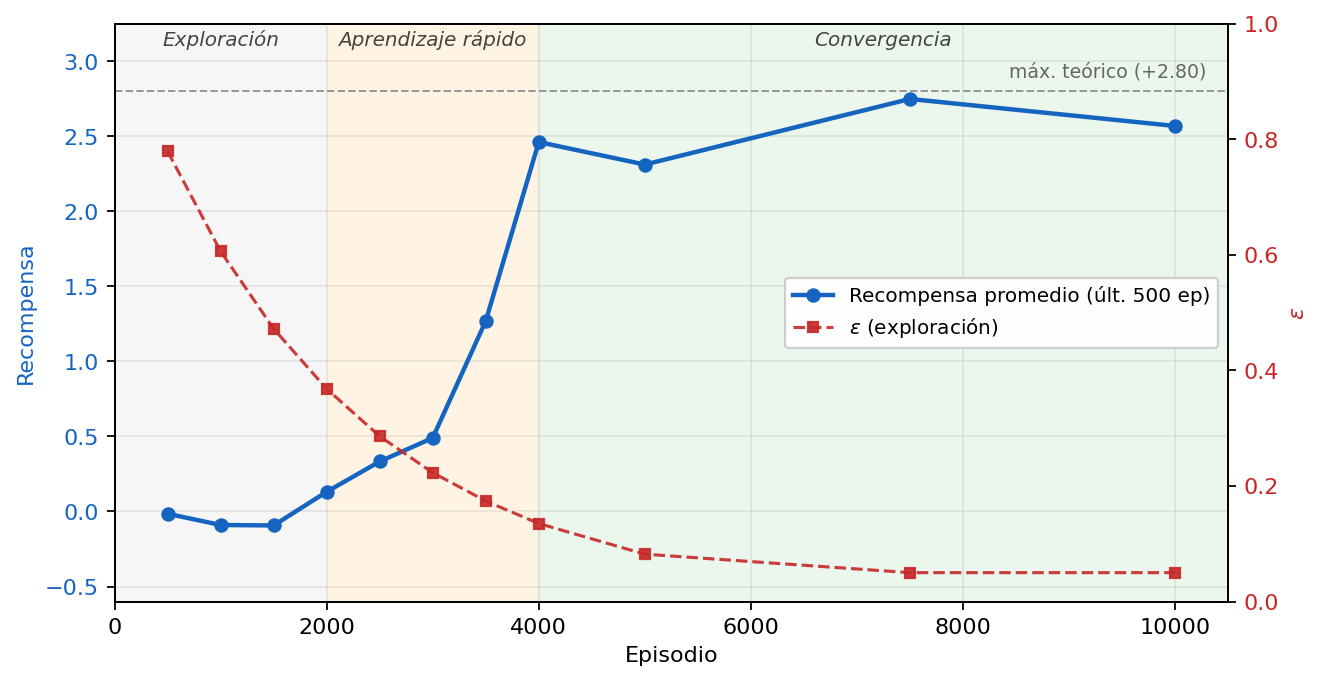
\includegraphics[width=0.85\linewidth]{minigrid_learning_curve.png}
  \caption{Recompensa promedio sobre los últimos 500 episodios (azul,
  eje izquierdo) y \(\varepsilon\) (rojo, eje derecho) en función del
  episodio. El sombreado de fondo separa las tres fases descritas en el
  texto. Datos del entrenamiento con \(\alpha=0.1\), \(\gamma=0.99\),
  \(\varepsilon: 1.0\to 0.05\) y decaimiento \(0.9995\).}
  \label{fig:learning_curve}
\end{figure}

% =====================================================================
\clearpage
\appendix
\section{Trabajo adicional: laberinto rectangular \texorpdfstring{$8\times 7$}{8x7}}
\label{ap:laberinto}

\textit{Este apéndice no forma parte de la respuesta a la rúbrica de la
entrega parcial. La rúbrica se refiere exclusivamente al ambiente
\texttt{MiniGrid-BlockedUnlockPickup-v0} descrito en el cuerpo principal.
Lo incluimos como trabajo adicional desarrollado en paralelo, por
trazabilidad con la discusión que se dio en el foro del curso.}

\subsection{Origen}

En el foro del curso se planteó como ejemplo un laberinto rectangular
\(8\times 7\) con muros internos en el que un agente debe ir de una celda
inicial a una celda objetivo. Lo trabajamos en paralelo al ambiente
principal, en parte por la discusión que se dio en el foro y en parte
porque el laberinto es un caso limpio para validar la implementación: la
solución óptima se obtiene de forma exacta con BFS, lo que da un punto de
referencia objetivo para comparar la política aprendida por Q-learning.

\subsection{Descripción}

El laberinto es una grilla de \num{8} filas por \num{7} columnas
(\num{56} celdas en total) con \num{65} segmentos de muro entre celdas
adyacentes (37 internos y 28 de borde). El agente parte en \((6,0)\) y
tiene que llegar a \((1,6)\). La distancia Manhattan entre ambas casillas
es \num{11}, pero los muros internos fuerzan rodeos que llevan el camino
mínimo a \num{25} pasos (verificado con BFS). El ambiente es determinista.

\subsection{Estados y acciones}

El estado es \(s = (x, y)\) con \(x\in\{0,\ldots,7\}\),
\(y\in\{0,\ldots,6\}\). Hay \(|\mathcal{S}|=56\). Las acciones son
\(\mathcal{A}=\{N, S, E, W\}\), todas siempre aplicables. Si la celda
destino existe y no hay muro entre la celda actual y la destino, el agente
se mueve. Si no, la acción es no-op: el agente se queda donde está y paga
el costo del paso.

\subsection{Recompensa}

\[
  R(s, a, s') =
  \begin{cases}
    +100 & s' = (1,6) \\
    -1   & \text{en cualquier otro caso}
  \end{cases}
\]
Es la formulación canónica de \emph{gridworld} con costo de paso uniforme.
Garantiza que la política óptima coincide exactamente con el camino más
corto medido en pasos.

\subsection{Resultados}

Q-learning tabular con \(\alpha=0.1\), \(\gamma=0.99\),
\(\varepsilon: 1.0\to 0.05\) y \num{2000} episodios produce una política
greedy que resuelve los \num{100} episodios de evaluación en \num{25} pasos
(igual al óptimo BFS) con retorno \(+76\). La Figura~\ref{fig:maze_greedy}
muestra el laberinto y el camino aprendido. La Figura~\ref{fig:maze_lc}
muestra la curva de aprendizaje.

\begin{figure}[!htbp]
  \centering
  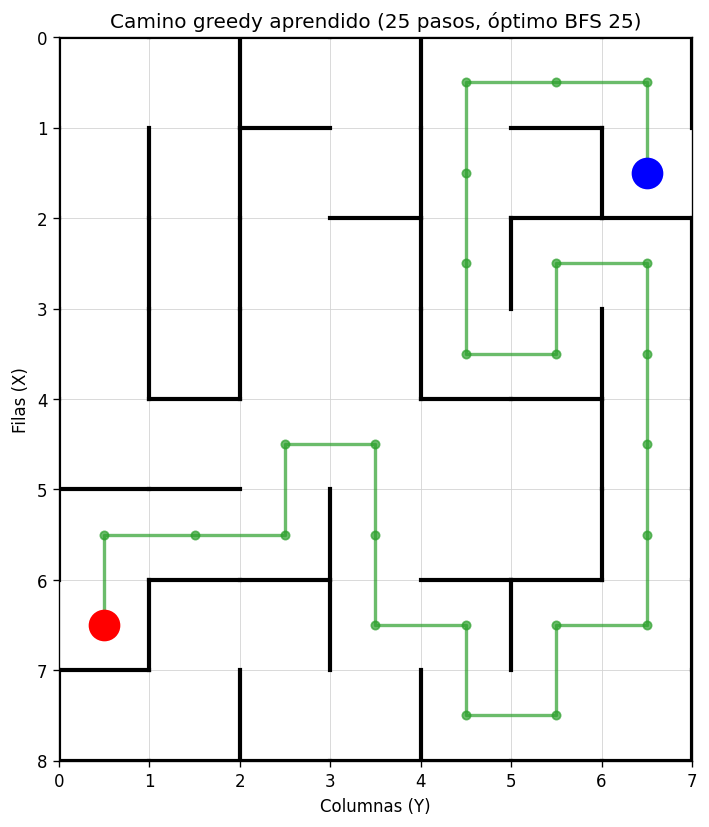
\includegraphics[width=0.55\linewidth]{maze_greedy_path.png}
  \caption{Laberinto y trayectoria greedy aprendida. Los 25 pasos coinciden
  con el óptimo de BFS.}
  \label{fig:maze_greedy}
\end{figure}

\begin{figure}[!htbp]
  \centering
  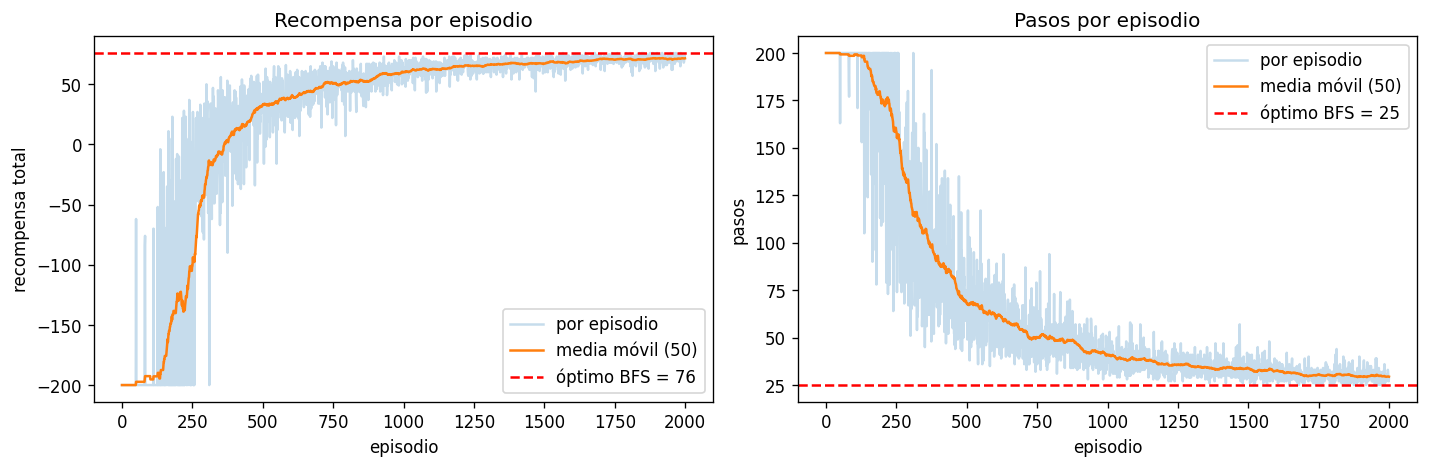
\includegraphics[width=0.85\linewidth]{maze_learning_curve.png}
  \caption{Curva de aprendizaje en el laberinto. El panel izquierdo muestra
  la recompensa por episodio; el derecho, el número de pasos por episodio.}
  \label{fig:maze_lc}
\end{figure}

\clearpage
% =====================================================================
\begin{thebibliography}{9}

\bibitem{sutton}
R. S. Sutton, A. G. Barto.
\emph{Reinforcement Learning: An Introduction}.
2.\textsuperscript{a} ed., MIT Press, 2018.

\bibitem{watkins}
C. J. C. H. Watkins, P. Dayan.
``Q-learning''.
\emph{Machine Learning}, vol.~8, n.\textsuperscript{o}~3, 1992.

\bibitem{minigrid}
M. Chevalier-Boisvert, B. Dai, M. Towers, R. de Lazcano, L. Willems, S.
Lahlou, S. Pal, P. S. Castro, J. Terry.
``Minigrid \& Miniworld: Modular \& Customizable Reinforcement Learning
Environments for Goal-Oriented Tasks''.
\emph{Advances in Neural Information Processing Systems (NeurIPS)}, 2023.

\end{thebibliography}

\end{document}
